\chapter{Concentration et dilution}\label{ch:g10:concentration-and-dilution}

Une poche de perfusion est suspendue au-dessus du lit d'un patient. Son
étiquette indique «~chlorure de sodium à 0.9~\%~»~: du sel dans de
l'eau, rien de plus. Pourtant, le nombre 0.9 n'est pas un détail. Trop
peu de sel, et les globules rouges du patient gonfleraient d'eau~; trop,
et ils se ratatineraient. Une solution ne se décrit pas seulement par
ses ingrédients, mais par la quantité de \omterm{def:g6:solutions-and-solubility:solute}{soluté} que contient chaque
volume de solution~: sa concentration. Ce chapitre mesure des
concentrations, prépare des solutions de concentration exacte, et les
dilue.

\begin{recall}
Une solution est formée d'un \omterm{def:g6:solutions-and-solubility:solute}{solvant} et d'un ou plusieurs \omterm{def:g6:solutions-and-solubility:solute}{solutés}
dissous~; la \omterm{def:g6:solutions-and-solubility:solubility}{solubilité} est la plus grande masse de \omterm{def:g6:solutions-and-solubility:solute}{soluté} qu'une
quantité donnée de \omterm{def:g6:solutions-and-solubility:solute}{solvant} peut dissoudre
(\cref{ch:g6:solutions-and-solubility}). La \omterm{def:g10:the-mole:amount}{quantité de matière} d'une
espèce vaut $n = m/M$, en \omterm{def:g10:the-mole:amount}{moles} (\cref{ch:g10:the-mole}).
\end{recall}

\begin{omfigure}
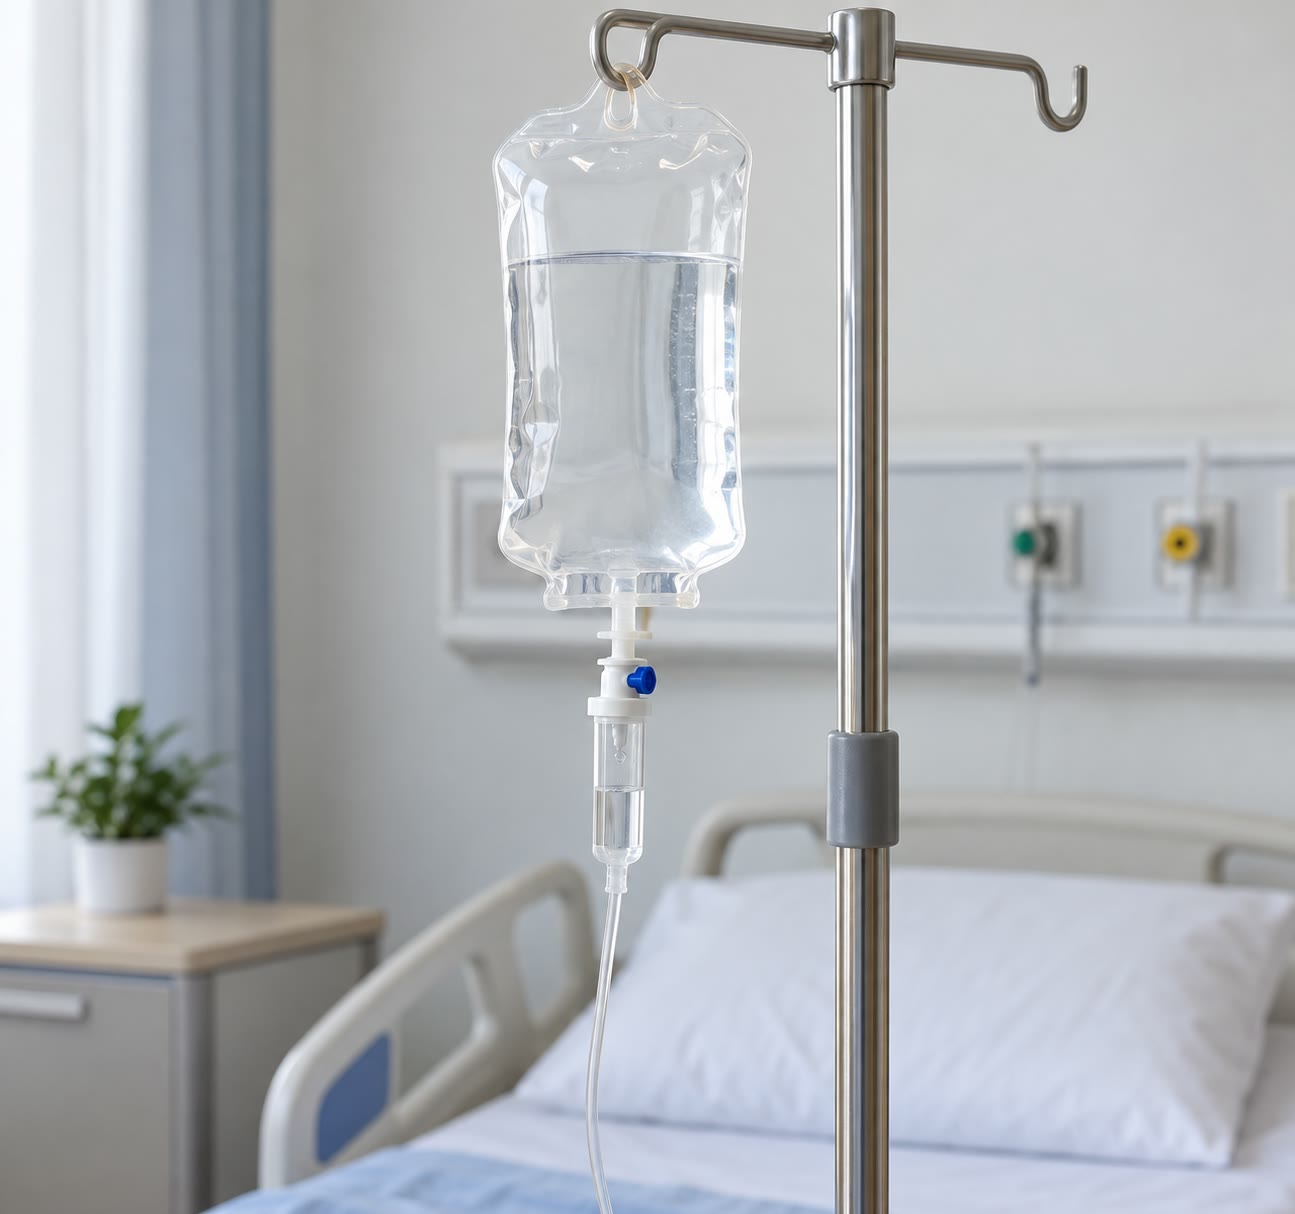
\includegraphics[width=0.42\linewidth]{images/book1/ai/g10-drip-bag.jpg}

{\small Une poche de perfusion de solution salée~: la concentration doit
être la bonne.}
\end{omfigure}

\section{La concentration massique}

\begin{definition}[Concentration massique]\label{def:g10:concentration-and-dilution:mass-concentration}
La \emph{concentration massique}\index{concentration massique} $C_m$ d'un
\omterm{def:g6:solutions-and-solubility:solute}{soluté} dans une solution est la masse de \omterm{def:g6:solutions-and-solubility:solute}{soluté} dissous par volume de
solution~:
\[
  C_m = \frac{m_{\text{soluté}}}{V_{\text{solution}}},
\]
en grammes par litre (\si{g/L}).
\end{definition}

\begin{example}[De l'eau sucrée]\label{ex:g10:concentration-and-dilution:sugar}
On dissout \qty{20}{g} de sucre dans de l'eau, et on complète la
solution à \qty{0.50}{L}. Sa \omterm{def:g10:concentration-and-dilution:mass-concentration}{concentration massique} en sucre est
$C_m = \qty{20}{g} / \qty{0.50}{L} = \qty{40}{g/L}$. Toute partie de
cette solution a la même concentration~: un verre de \qty{0.20}{L}
contient $\qty{40}{g/L} \times \qty{0.20}{L} = \qty{8.0}{g}$ de sucre.
\end{example}


\begin{remark}[Le volume est celui de la solution]\label{rem:g10:concentration-and-dilution:volume}
Le volume qui figure dans $C_m$ est celui de toute la solution, et non
celui de l'eau versée~: la dissolution d'un \omterm{def:g6:solutions-and-solubility:solute}{soluté} modifie un peu le
volume. C'est pourquoi on \emph{complète} toujours une solution jusqu'à
un volume final connu, dans une fiole jaugée prévue à cet effet.
\end{remark}

\begin{remark}[Concentration n'est pas solubilité]\label{rem:g10:concentration-and-dilution:not-solubility}
% ledger: sol:NaCl, saline:NaCl
La \omterm{def:g6:solutions-and-solubility:solubility}{solubilité} d'un \omterm{def:g6:solutions-and-solubility:solute}{soluté} est la concentration la \emph{plus grande}
qu'il puisse atteindre~; une solution peut avoir n'importe quelle
concentration comprise entre zéro et cette valeur. Le chlorure de sodium
\omterm{def:g2:mixing-and-dissolving:dissolve}{se dissout} jusqu'à environ \qty{360}{g} par kilogramme d'eau à
\qty{25}{\celsius}~; la poche de perfusion n'en contient que \qty{9}{g}
par litre, très loin de la saturation.
\end{remark}

\begin{remark}[Les pourcentages des étiquettes]\label{rem:g10:concentration-and-dilution:percent}
% ledger: saline:NaCl
Sur les étiquettes médicales et alimentaires, «~0.9~\%~» pour un solide
dissous dans l'eau signifie en général \qty{0.9}{g} de \omterm{def:g6:solutions-and-solubility:solute}{soluté} pour
\qty{100}{mL} de solution. En grammes par litre, c'est dix fois plus~:
la poche contient \qty{9.0}{g/L} de chlorure de sodium.
\end{remark}

\section{La concentration molaire}

\begin{definition}[Concentration molaire]\label{def:g10:concentration-and-dilution:molar-concentration}
La \emph{concentration molaire}\index{concentration molaire} $c$ d'un
\omterm{def:g6:solutions-and-solubility:solute}{soluté} dans une solution est la quantité de \omterm{def:g6:solutions-and-solubility:solute}{soluté} dissous par volume de
solution~:
\[
  c = \frac{n_{\text{soluté}}}{V_{\text{solution}}},
\]
en \omterm{def:g10:the-mole:amount}{moles} par litre (\si{mol/L}).
\end{definition}

\begin{proposition}[D'une concentration à l'autre]\label{prop:g10:concentration-and-dilution:link}
Pour un \omterm{def:g6:solutions-and-solubility:solute}{soluté} de \omterm{def:g10:the-mole:molar-mass}{masse molaire} $M$,
\[
  C_m = c \times M .
\]
\end{proposition}

\begin{proof}
$C_m = m / V = (n \times M) / V = (n / V) \times M = c \times M$.
\end{proof}

\begin{example}[La poche de perfusion en moles]\label{ex:g10:concentration-and-dilution:drip}
% ledger: saline:NaCl, saline:Na, aw:Na, aw:Cl
La poche contient \qty{9.0}{g/L} de chlorure de sodium, de \omterm{def:g10:the-mole:molar-mass}{masse molaire}
\qty{58.5}{g/mol}. Sa \omterm{def:g10:concentration-and-dilution:molar-concentration}{concentration molaire} est
\[
  c = \frac{C_m}{M} = \frac{\qty{9.0}{g/L}}{\qty{58.5}{g/mol}}
    = \qty{0.154}{mol/L}.
\]
L'étiquette du fabricant donne le même nombre, présenté autrement~: 154
millièmes de \omterm{def:g10:the-mole:amount}{mole} d'\omterm{def:g9:ions:ion}{ions} sodium par litre.
\end{example}

\begin{remark}[Les ions en solution]\label{rem:g10:concentration-and-dilution:ions}
Le chlorure de sodium \omterm{def:g2:mixing-and-dissolving:dissolve}{se dissout} sous forme d'\omterm{def:g9:ions:ion}{ions} séparés \ce{Na+} et
\ce{Cl-} (\cref{ch:g9:ions})~: une solution de chlorure de sodium à
\qty{0.154}{mol/L} contient \qty{0.154}{mol/L} d'\omterm{def:g9:ions:ion}{ions} sodium et
\qty{0.154}{mol/L} d'\omterm{def:g9:ions:ion}{ions} chlorure. La façon dont un solide ionique se
défait dans l'eau est l'objet d'un chapitre suivant.
\end{remark}

\begin{omfigure}
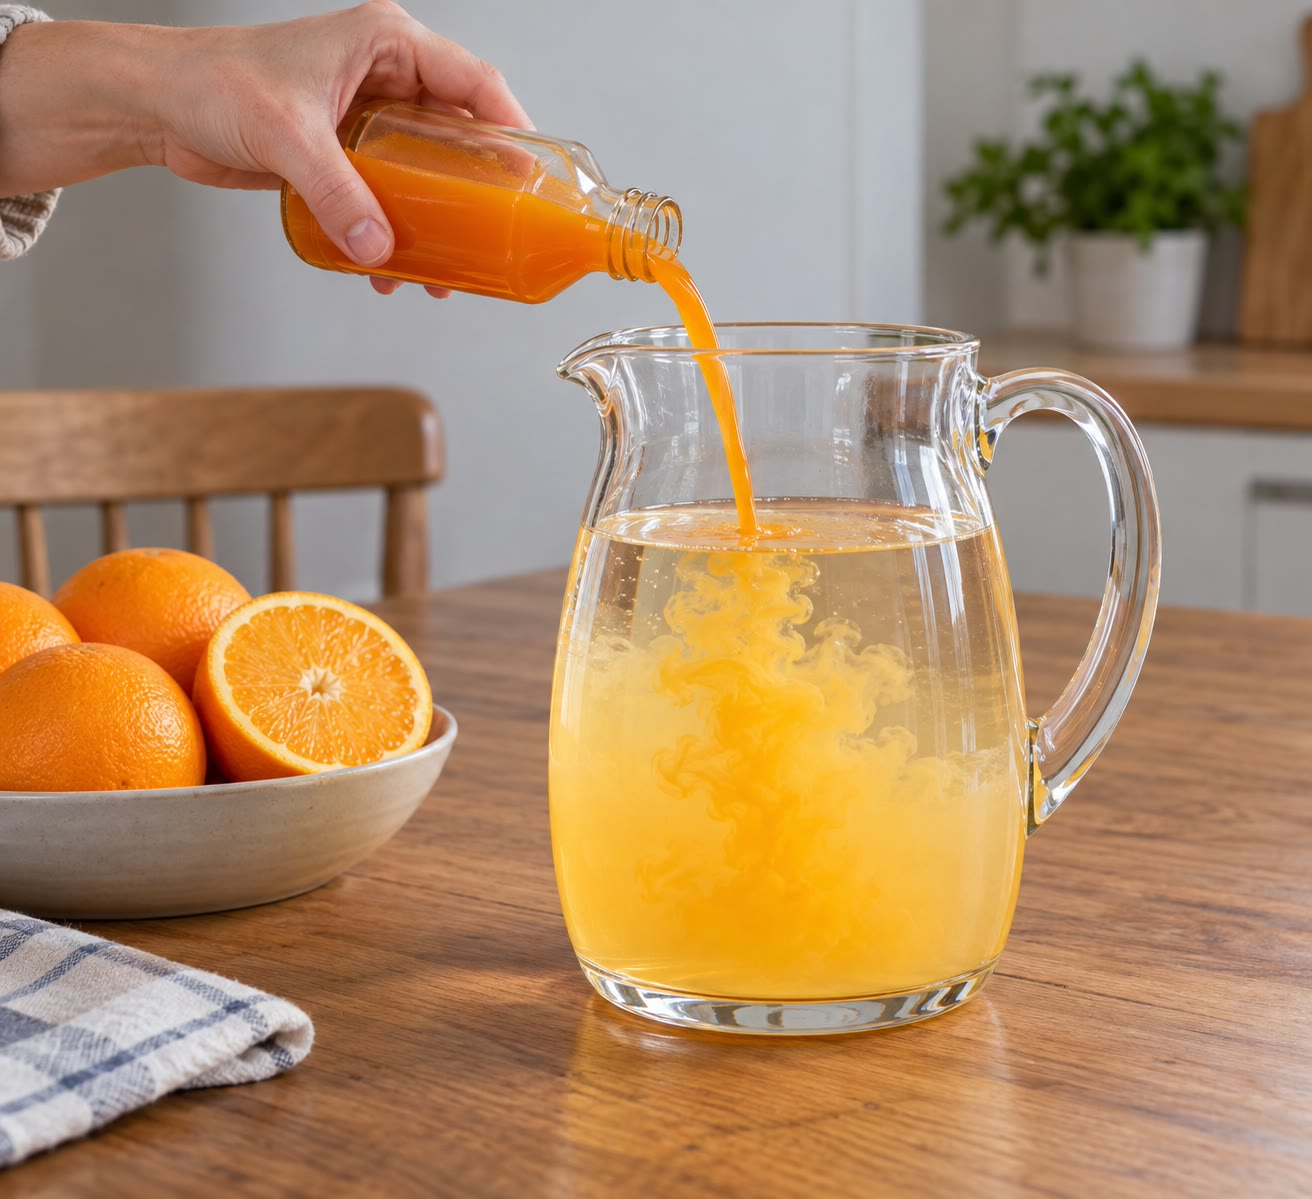
\includegraphics[width=0.45\linewidth]{images/book1/ai/g10-squash-jug.jpg}

{\small Du sirop dilué avec de l'eau dans une carafe~: la boisson
contient la même quantité de sirop de fruit, dans un volume plus
grand.}
\end{omfigure}

\section{Préparer une solution par dissolution}

\begin{method}[Préparer une solution par dissolution d'un solide]\label{met:g10:concentration-and-dilution:dissolving}
Pour préparer un volume $V$ de solution de \omterm{def:g10:concentration-and-dilution:molar-concentration}{concentration molaire} $c$~:
\begin{enumerate}
  \item Calculer la \omterm{def:g10:the-mole:amount}{quantité de matière} nécessaire, $n = c \times V$, et
        la masse à peser, $m = n \times M$.
  \item Peser cette masse de solide dans une coupelle sur une balance.
  \item Verser le solide à l'aide d'un entonnoir dans une fiole jaugée de
        volume $V$~; rincer la coupelle et l'entonnoir à l'eau distillée
        au-dessus de la fiole, pour ne perdre aucune trace de solide.
  \item Ajouter de l'eau distillée jusqu'à la moitié environ de la fiole
        et agiter jusqu'à dissolution complète du solide.
  \item Compléter avec de l'eau distillée jusqu'au trait de jauge, les
        dernières gouttes au compte-gouttes~; boucher la fiole et la
        retourner plusieurs fois pour homogénéiser.
\end{enumerate}
\end{method}

\begin{omfigure}
\begin{tikzpicture}[font=\small, scale=1.05]
  % 1. weigh
  \pic[transform shape] at (0,0) {balance};
  \fill[black!8, draw=black!55] (-0.45,0.8) -- (0.45,0.8) -- (0.38,0.98)
    -- (-0.38,0.98) -- cycle;
  \fill[white, draw=black!40] (-0.25,0.98) .. controls (-0.1,1.15) and
    (0.1,1.15) .. (0.25,0.98) -- cycle;
  \node[align=center, anchor=north] at (0,-0.2) {1. peser\\ le solide};
  % 2. transfer through a funnel
  \pic[transform shape] at (3.2,0) {volflask={0.08}{omWater}};
  \pic[transform shape] at (3.2,3.0) {funnel};
  \draw[omProp, thick, -{Stealth}] (2.4,5.0) -- (2.85,4.65);
  \node[align=center, anchor=north] at (3.2,-0.2) {2. transvaser,\\ rincer};
  % 3. half full, swirl
  \pic[transform shape] at (6.4,0) {volflask={0.45}{omWater}};
  \draw[omProp, thick, -{Stealth}] (5.55,0.5) arc[start angle=200,
    end angle=340, x radius=0.9, y radius=0.3];
  \node[align=center, anchor=north] at (6.4,-0.2) {3. à moitié~:\\ agiter pour\\ dissoudre};
  % 4. to the mark
  \pic[transform shape] at (9.6,0) {volflask={1}{omWater}};
  \fill[black!45] (9.43,3.6) rectangle (9.77,3.85);
  \draw[omDef, thick, <-] (9.82,2.9) -- (10.6,3.3) node[right] {trait de jauge};
  \node[align=center, anchor=north] at (9.6,-0.2) {4. compléter,\\
    boucher,\\ homogénéiser};
\end{tikzpicture}

{\small Préparer une solution par dissolution d'un solide~: peser,
transvaser, dissoudre, puis compléter jusqu'au trait de jauge de la
fiole.}
\end{omfigure}

\begin{inthelab}[Ajuster au trait de jauge]
Le trait de jauge d'une fiole jaugée est un anneau gravé autour de son
col. L'eau, dans un tube de verre étroit, ne se termine pas à plat~: sa
surface se creuse au milieu et forme un ménisque. La fiole est remplie
quand le \emph{bas} du ménisque affleure le trait, l'œil étant à la
hauteur du trait, de sorte que l'avant et l'arrière de l'anneau se
confondent en une seule ligne. Vu d'en haut ou d'en bas, le niveau peut
sembler juste alors qu'il ne l'est pas.
\end{inthelab}

\begin{omfigure}
\begin{tikzpicture}[font=\small]
  \newcommand{\neck}[2]{% x, meniscus bottom height
    \fill[omWater] (#1-0.5,0) -- (#1-0.5,{#2+0.25}) .. controls
      (#1-0.25,#2) and (#1+0.25,#2) .. (#1+0.5,{#2+0.25}) -- (#1+0.5,0) -- cycle;
    \draw[black!60, line width=0.8pt] (#1-0.5,0) -- (#1-0.5,3);
    \draw[black!60, line width=0.8pt] (#1+0.5,0) -- (#1+0.5,3);
    \draw[omDef, line width=0.9pt] (#1-0.5,1.5) -- (#1+0.5,1.5);
    \draw[black!50] (#1-0.5,{#2+0.25}) .. controls (#1-0.25,#2) and
      (#1+0.25,#2) .. (#1+0.5,{#2+0.25});}
  \newcommand{\eye}[2]{% x, y: an eye looking to the right
    \draw[black!70] (#1-0.25,#2) .. controls (#1-0.1,#2+0.18) and
      (#1+0.1,#2+0.18) .. (#1+0.2,#2) .. controls (#1+0.1,#2-0.18) and
      (#1-0.1,#2-0.18) .. (#1-0.25,#2);
    \fill[black!70] (#1+0.05,#2) circle (0.06);}
  % right
  \neck{1.5}{1.5}
  \eye{-0.4}{1.5}
  \draw[dashed, black!50] (-0.1,1.5) -- (2.4,1.5);
  \node[align=center] at (1.5,-0.55) {correct~: œil au niveau,\\ bas du ménisque sur le trait};
  % too high
  \neck{6}{1.85}
  \eye{4.1}{1.85}
  \draw[dashed, black!50] (4.4,1.85) -- (6.9,1.85);
  \node[align=center] at (6,-0.55) {trop d'eau~:\\ ménisque au-dessus};
  % too low
  \neck{10.5}{0.85}
  \eye{8.6}{0.85}
  \draw[dashed, black!50] (8.9,0.85) -- (11.4,0.85);
  \node[align=center] at (10.5,-0.55) {pas assez d'eau~:\\ ménisque au-dessous};
\end{tikzpicture}

{\small Le col d'une fiole jaugée, agrandi et vu avec l'œil à la hauteur
du ménisque. La ligne bleue est le trait de jauge. Seule la fiole de
gauche est remplie correctement.}
\end{omfigure}

\section{Diluer}

\begin{definition}[Dilution, solution mère, facteur de dilution]\label{def:g10:concentration-and-dilution:dilution}
Une \emph{dilution}\index{dilution} diminue la concentration d'une
solution par ajout de \omterm{def:g6:solutions-and-solubility:solute}{solvant}. La solution concentrée prélevée au départ
est la \emph{solution mère}\index{solution mere@solution mère}. Le \emph{facteur de
dilution}\index{facteur de dilution} $F$ est le rapport de la
concentration de la solution mère à celle de la solution diluée~:
\[
  F = \frac{c_{\text{mère}}}{c_{\text{fille}}} .
\]
\end{definition}

\begin{proposition}[La quantité de soluté se conserve]\label{prop:g10:concentration-and-dilution:kept}
Au cours d'une \omterm{def:g10:concentration-and-dilution:dilution}{dilution}, la quantité de \omterm{def:g6:solutions-and-solubility:solute}{soluté} ne change pas~: si un
volume $V_0$ de \omterm{def:g10:concentration-and-dilution:dilution}{solution mère} de concentration $c_0$ est complété jusqu'à
un volume $V_1$, la solution diluée a la concentration $c_1$ donnée par
\[
  c_0 \times V_0 = c_1 \times V_1,
  \qquad\text{donc}\qquad
  F = \frac{c_0}{c_1} = \frac{V_1}{V_0} .
\]
Il en va de même pour les \omterm{def:g10:concentration-and-dilution:mass-concentration}{concentrations massiques}.
\end{proposition}

\begin{proof}
On n'ajoute que du \omterm{def:g6:solutions-and-solubility:solute}{solvant}~: le \omterm{def:g6:solutions-and-solubility:solute}{soluté} prélevé avec le volume $V_0$, une
quantité $c_0 V_0$, se retrouve tout entier dans le volume final $V_1$,
où il représente la quantité $c_1 V_1$.
\end{proof}


\begin{method}[Préparer une solution par dilution]\label{met:g10:concentration-and-dilution:diluting}
Pour préparer un volume $V_1$ de solution de concentration $c_1$ à partir
d'une \omterm{def:g10:concentration-and-dilution:dilution}{solution mère} de concentration $c_0$~:
\begin{enumerate}
  \item Calculer le volume de \omterm{def:g10:concentration-and-dilution:dilution}{solution mère} à prélever,
        $V_0 = c_1 V_1 / c_0$ (c'est-à-dire $V_1 / F$).
  \item Verser un peu de \omterm{def:g10:concentration-and-dilution:dilution}{solution mère} dans un bécher propre (on ne
        pipette jamais directement dans le flacon) et prélever exactement
        $V_0$ avec une pipette jaugée, remplie jusqu'à son trait.
  \item Vider la pipette dans une fiole jaugée de volume $V_1$.
  \item Compléter avec de l'eau distillée jusqu'au trait de jauge,
        boucher et homogénéiser.
\end{enumerate}
\end{method}

\begin{example}[Une dilution au dixième]\label{ex:g10:concentration-and-dilution:tenfold}
Une \omterm{def:g10:concentration-and-dilution:dilution}{solution mère} de sulfate de cuivre a $c_0 = \qty{0.10}{mol/L}$~; il
faut \qty{100.0}{mL} à $c_1 = \qty{0.010}{mol/L}$. Le \omterm{def:g10:concentration-and-dilution:dilution}{facteur de
dilution} vaut $F = 0.10 / 0.010 = 10$, donc $V_0 = \qty{100.0}{mL} / 10 =
\qty{10.0}{mL}$~: une pipette de \qty{10.0}{mL} et une fiole de
\qty{100.0}{mL}.
\end{example}

\begin{omfigure}
\begin{tikzpicture}[font=\small, scale=0.85]
  % 1. take the stock with a pipette
  \pic[transform shape] at (0,0) {beaker={0.6}{cyan!70!blue!55}};
  \pic[transform shape] at (0,0.2) {pipette={1}{cyan!70!blue!55}};
  \node[align=center, anchor=north] at (0,-0.2) {1. pipeter $V_0$\\ de solution mère};
  \draw[omProp, very thick, -{Stealth}] (1.3,2.6) -- (2.6,2.6);
  % 2. empty it into the flask
  \pic[transform shape] at (4,0) {volflask={0.22}{cyan!70!blue!55}};
  \pic[transform shape] at (4,2.6) {pipette={0.12}{cyan!70!blue!55}};
  \node[align=center, anchor=north] at (4,-0.2) {2. la vider dans\\ la fiole};
  \draw[omProp, very thick, -{Stealth}] (5.3,2.6) -- (6.6,2.6);
  % 3. water to the mark
  \pic[transform shape] at (8,0) {volflask={1}{cyan!70!blue!14}};
  \draw[omDef, thick, <-] (8.2,2.9) -- (9.1,3.4) node[right] {trait de jauge};
  \node[align=center, anchor=north] at (8,-0.2) {3. eau jusqu'au trait~:\\
    volume $V_1$};
\end{tikzpicture}

{\small Diluer~: un volume $V_0$ de \omterm{def:g10:concentration-and-dilution:dilution}{solution mère}, mesuré à la pipette,
est complété à $V_1$ dans une fiole jaugée. La couleur pâlit du \omterm{def:g10:concentration-and-dilution:dilution}{facteur
de dilution} $V_1 / V_0$.}
\end{omfigure}

\section{Une échelle de teintes}

\begin{definition}[Solution étalon, échelle de teintes]\label{def:g10:concentration-and-dilution:standard}
Une \emph{solution étalon}\index{solution etalon@solution étalon} est une solution dont
la concentration est connue avec précision. Une \emph{échelle de
teintes}\index{echelle de teintes@échelle de teintes} est une série de solutions étalons
du même \omterm{def:g6:solutions-and-solubility:solute}{soluté}, de concentrations croissantes, préparées en général par
\omterm{def:g10:concentration-and-dilution:dilution}{dilution} d'une même \omterm{def:g10:concentration-and-dilution:dilution}{solution mère}~; comparer une solution inconnue à
cette échelle donne une estimation de sa concentration.
\end{definition}

\begin{example}[Une échelle de bleus]\label{ex:g10:concentration-and-dilution:scale}
À partir d'une \omterm{def:g10:concentration-and-dilution:dilution}{solution mère} de sulfate de cuivre à \qty{0.20}{mol/L},
on prépare six étalons à 0.02, 0.04, 0.06, 0.08, 0.10 et
\qty{0.12}{mol/L}, chacun dans des tubes identiques remplis à la même
hauteur. Une solution de concentration inconnue, dans le même type de
tube, paraît plus foncée que le tube à \qty{0.06}{mol/L} et plus claire
que celui à \qty{0.08}{mol/L}~: sa concentration est comprise entre les
deux, environ \qty{0.07}{mol/L}.
\end{example}

\begin{omfigure}
\begin{tikzpicture}[font=\small]
  \foreach \i/\c/\p in {0/0.02/8, 1/0.04/16, 2/0.06/24, 3/0.08/32,
                        4/0.10/40, 5/0.12/48} {
    \pic at (1.2*\i,0) {testtube={0.75}{cyan!70!blue!\p}};
    \node[anchor=north] at (1.2*\i,-0.15) {\c};
  }
  \pic at (8.4,0) {testtube={0.75}{cyan!70!blue!28}};
  \node[anchor=north] at (8.4,-0.15) {?};
  \draw[black!40] (7.55,-0.6) -- (7.55,3.2);
  \node[anchor=north] at (3,-0.7) {concentration (\si{mol/L})};
  \node[anchor=north] at (8.4,-0.7) {inconnue};
\end{tikzpicture}

{\small Une \omterm{def:g10:concentration-and-dilution:standard}{échelle de teintes} de solutions de sulfate de cuivre et une
solution inconnue. L'inconnue se situe entre le troisième et le
quatrième tube.}
\end{omfigure}

\begin{safety}{\ghs[0.82cm]{GHS05}\ghs[0.82cm]{GHS07}\ghs[0.82cm]{GHS09}}
% ledger: ghs:CuSO4
Les solutions de sulfate de cuivre sont nocives en cas d'ingestion,
irritantes pour la peau, dangereuses pour les yeux et très toxiques pour
les organismes aquatiques. Lunettes et gants~; les solutions usagées
sont récupérées pour être traitées, jamais versées dans l'évier.
\end{safety}

\begin{remark}[Les limites de l'œil]\label{rem:g10:concentration-and-dilution:eye}
L'œil ne peut dire que «~entre ces deux tubes~». Pour mesurer plus
finement une concentration à partir de la couleur d'une solution, les
chimistes mesurent la quantité de lumière qu'elle absorbe~; un chapitre
suivant fait exactement cela.
\end{remark}

\section{Exercices}

\begin{exercise}[$\star$]\label{exo:g10:concentration-and-dilution:1}
On dissout \qty{5.0}{g} de sucre pour obtenir \qty{250}{mL} de
solution. Calculer la \omterm{def:g10:concentration-and-dilution:mass-concentration}{concentration massique} en sucre, en grammes par
litre.
\end{exercise}

\begin{exercise}[$\star$]\label{exo:g10:concentration-and-dilution:2}
Une solution de \qty{200}{mL} contient \qty{0.050}{mol} de glucose.
Calculer sa \omterm{def:g10:concentration-and-dilution:molar-concentration}{concentration molaire}.
\end{exercise}

\begin{exercise}[$\star$]\label{exo:g10:concentration-and-dilution:3}
Quelle masse de sulfate de cuivre anhydre \ce{CuSO4} faut-il peser pour
préparer \qty{100.0}{mL} de solution à \qty{0.10}{mol/L}~?
\end{exercise}

\begin{exercise}[$\star$]\label{exo:g10:concentration-and-dilution:4}
On dilue une \omterm{def:g10:concentration-and-dilution:dilution}{solution mère} à \qty{1.0}{mol/L} jusqu'à \qty{0.050}{mol/L}.
Quel est le \omterm{def:g10:concentration-and-dilution:dilution}{facteur de dilution}~? Quel volume de \omterm{def:g10:concentration-and-dilution:dilution}{solution mère} faut-il
pour préparer \qty{100.0}{mL} de solution diluée~?
\end{exercise}

\begin{exercise}[$\star$]\label{exo:g10:concentration-and-dilution:5}
Une solution de chlorure de sodium a une \omterm{def:g10:concentration-and-dilution:molar-concentration}{concentration molaire} de
\qty{0.10}{mol/L}. Quelle est sa \omterm{def:g10:concentration-and-dilution:mass-concentration}{concentration massique}~?
\end{exercise}

\begin{exercise}[$\star\star$]\label{exo:g10:concentration-and-dilution:6}
Quel volume d'une \omterm{def:g10:concentration-and-dilution:dilution}{solution mère} à \qty{0.50}{mol/L} faut-il prélever
pour préparer \qty{250.0}{mL} de solution à \qty{0.020}{mol/L}~?
Nommer les deux pièces de verrerie utilisées.
\end{exercise}

\begin{exercise}[$\star\star$]\label{exo:g10:concentration-and-dilution:7}
Pourquoi prépare-t-on une solution de concentration exacte dans une
fiole jaugée plutôt que dans un bécher gradué~? Pourquoi mesure-t-on un
volume de \omterm{def:g10:concentration-and-dilution:dilution}{solution mère} avec une pipette jaugée plutôt qu'avec une
éprouvette graduée~?
\end{exercise}

\begin{exercise}[$\star\star$]\label{exo:g10:concentration-and-dilution:8}
Observer l'\omterm{def:g10:concentration-and-dilution:standard}{échelle de teintes} du sulfate de cuivre. Une seconde solution
inconnue est plus claire que le tube à \qty{0.04}{mol/L} mais plus
foncée que celui à \qty{0.02}{mol/L}. Estimer sa concentration. Comment
pourrait-on modifier l'échelle pour l'estimer plus précisément~?
\end{exercise}

\begin{exercise}[$\star\star$]\label{exo:g10:concentration-and-dilution:9}
Une solution de glucose pour perfusion contient \qty{50}{g/L} de glucose
\ce{C6H12O6}. Calculer sa \omterm{def:g10:concentration-and-dilution:molar-concentration}{concentration molaire}.
\end{exercise}

\begin{exercise}[$\star\star$]\label{exo:g10:concentration-and-dilution:10}
On prépare un sirop en dissolvant \qty{342}{g} de saccharose
\ce{C12H22O11} pour obtenir \qty{1.00}{L} de solution. Calculer sa
\omterm{def:g10:concentration-and-dilution:molar-concentration}{concentration molaire}. On le dilue ensuite dix fois. Quelle masse de
saccharose contient une cuillerée de \qty{20}{mL} du sirop dilué~?
\end{exercise}

\begin{exercise}[$\star\star$]\label{exo:g10:concentration-and-dilution:11}
Une solution a une \omterm{def:g10:concentration-and-dilution:mass-concentration}{concentration massique} de \qty{12}{g/L}. Quelle est
sa concentration (a) après ajout d'eau doublant son volume~; (b) après
\omterm{def:g3:separating-mixtures:evaporate}{évaporation} de la moitié de son eau, tout le \omterm{def:g6:solutions-and-solubility:solute}{soluté} restant dissous~?
\end{exercise}

\begin{exercise}[$\star\star\star$]\label{exo:g10:concentration-and-dilution:12}
On dilue dix fois une solution à \qty{0.10}{mol/L}, puis on dilue encore
dix fois le résultat, et une fois de plus.
\begin{enumerate}
  \item Quelle est la concentration finale~?
  \item Pourquoi procède-t-on en trois étapes plutôt qu'en une seule
        \omterm{def:g10:concentration-and-dilution:dilution}{dilution} par 1000 (penser aux volumes de verrerie nécessaires)~?
\end{enumerate}
\end{exercise}

\begin{exercise}[$\star\star\star$]\label{exo:g10:concentration-and-dilution:13}
On dissout \qty{11.1}{g} de chlorure de calcium \ce{CaCl2} pour obtenir
\qty{500.0}{mL} de solution. Dans l'eau, le solide se sépare en \omterm{def:g9:ions:ion}{ions}
calcium \ce{Ca^2+} et en \omterm{def:g9:ions:ion}{ions} chlorure \ce{Cl-}.
\begin{enumerate}
  \item Calculer la \omterm{def:g10:concentration-and-dilution:molar-concentration}{concentration molaire} du chlorure de calcium dissous.
  \item En déduire les \omterm{def:g10:concentration-and-dilution:molar-concentration}{concentrations molaires} des \omterm{def:g9:ions:ion}{ions} calcium et des
        \omterm{def:g9:ions:ion}{ions} chlorure dans la solution.
\end{enumerate}
\end{exercise}

\begin{exercise}[$\star\star\star$]\label{exo:g10:concentration-and-dilution:14}
Le col d'une fiole jaugée de \qty{100.0}{mL} a un diamètre intérieur de
\qty{1.2}{cm}. Un élève la remplit avec le bas du ménisque
\qty{2}{mm} au-dessus du trait.
\begin{enumerate}
  \item Quel volume d'eau supplémentaire a-t-il ajouté (volume d'un
        cylindre~: $\pi r^2 h$)~?
  \item De quel pourcentage la concentration de la solution est-elle
        trop faible~?
\end{enumerate}
\end{exercise}

\begin{exercise}[$\star\star\star$]\label{exo:g10:concentration-and-dilution:15}
On \omterm{def:g6:pure-substances-and-mixtures:mixture}{mélange} \qty{100}{mL} de solution de chlorure de sodium à
\qty{0.20}{mol/L} avec \qty{300}{mL} de solution de chlorure de sodium
à \qty{0.10}{mol/L}. En supposant que les volumes s'additionnent,
calculer la concentration du \omterm{def:g6:pure-substances-and-mixtures:mixture}{mélange}. Est-ce la moyenne des deux
concentrations~? Expliquer.
\end{exercise}

\section{Problème~: la poche de perfusion}

\begin{problem}[{Problème du week-end --- quelle quantité d'une solution
salée concentrée entre dans une poche de sérum physiologique «~à
0.9~\%~»~?}]
\label{pb:g10:concentration-and-dilution:1}
% ledger: saline:NaCl, saline:Na, sol:NaCl, aw:Na, aw:Cl, const:NA
Le laboratoire de la pharmacie d'un hôpital dispose d'une solution
stérile concentrée de chlorure de sodium à \qty{200}{g/L} (sur son
étiquette~: «~20~\%~»). Il doit préparer des poches de \qty{500}{mL} de
la solution «~à 0.9~\%~» utilisée en perfusion, en diluant la solution
concentrée avec de l'eau stérile.

\medskip
\noindent\textbf{Partie I --- Ce que signifie 0.9~\%.}
\begin{enumerate}
  \item L'étiquette «~0.9~\%~» signifie \qty{0.9}{g} de sel pour
        \qty{100}{mL} de solution. Donner la \omterm{def:g10:concentration-and-dilution:mass-concentration}{concentration massique} en
        \si{g/L}.
  \item L'exprimer aussi en milligrammes par millilitre.
  \item Quelle masse de chlorure de sodium une poche de \qty{500}{mL}
        contient-elle~?
  \item Le chlorure de sodium \omterm{def:g2:mixing-and-dissolving:dissolve}{se dissout} jusqu'à environ \qty{360}{g} par
        kilogramme d'eau. La solution de la poche est-elle loin de la
        saturation~?
  \item Un patient reçoit \qty{1.0}{L} de cette solution en une journée.
        Quelle masse de sel cela représente-t-il~?
\end{enumerate}

\medskip
\noindent\textbf{Partie II --- En \omterm{def:g10:the-mole:amount}{moles}.}
\begin{enumerate}[resume]
  \item Calculer la \omterm{def:g10:the-mole:molar-mass}{masse molaire} du chlorure de sodium.
  \item Calculer la \omterm{def:g10:concentration-and-dilution:molar-concentration}{concentration molaire} de la solution de la poche.
  \item Quelle quantité de chlorure de sodium une poche contient-elle~?
  \item Quelles sont les \omterm{def:g10:concentration-and-dilution:molar-concentration}{concentrations molaires} des \omterm{def:g9:ions:ion}{ions} sodium et des
        \omterm{def:g9:ions:ion}{ions} chlorure dans la poche~?
  \item Combien d'\omterm{def:g9:ions:ion}{ions} sodium une poche contient-elle~?
\end{enumerate}

\medskip
\noindent\textbf{Partie III --- À partir de la solution concentrée.}
\begin{enumerate}[resume]
  \item Calculer le \omterm{def:g10:concentration-and-dilution:dilution}{facteur de dilution} entre la solution concentrée et
        la solution de la poche.
  \item Quelle masse de chlorure de sodium doit provenir de la solution
        concentrée pour une poche~? En déduire le volume de solution
        concentrée à prélever.
  \item Vérifier ce volume à l'aide du \omterm{def:g10:concentration-and-dilution:dilution}{facteur de dilution}.
  \item Calculer la \omterm{def:g10:concentration-and-dilution:molar-concentration}{concentration molaire} de la solution concentrée, et
        vérifier que $c_0 V_0 = c_1 V_1$.
  \item Quel volume d'eau stérile ajoute-t-on alors, environ (on suppose
        que les volumes s'additionnent)~?
\end{enumerate}

\medskip
\noindent\textbf{Partie IV --- Verrerie et précision.}
\begin{enumerate}[resume]
  \item Il n'existe pas de pipette jaugée de ce volume. Quelle pièce de
        verrerie, graduée au dixième de millilitre, pourrait le
        délivrer~?
  \item Dans quel récipient faut-il ajuster le volume final pour qu'il
        soit précis~?
  \item Si l'on prélevait \qty{23.0}{mL} au lieu du bon volume, quelle
        \omterm{def:g10:concentration-and-dilution:mass-concentration}{concentration massique} aurait la poche~? De quel pourcentage
        serait-elle fausse~?
  \item Donner la réponse finale~: quel volume de solution concentrée
        entre dans une poche de \qty{500}{mL}~?
\end{enumerate}
\end{problem}
